\section{Categorisation of the non-VBF production modes}
\label{sec:htoinv_categorisation}

% This section is up-to-date as of 15th May.

To extract maximum sensitivity to the \higgstoinv decay from the analysis, categories are established to target each of the production modes. From first principles, the topologies outlined in Chpt.~\ref{subsec:theory_higgs_production_modes} provide an initial direction of the expected structure. Steps are taken to ensure the categories that target the production mechanism---and the subcategories that capitalise on specific topologies within the mechanism---are orthogonal. An additional angular variable cut based on optimisation studies in Chpt.~\ref{subsec:htoinv_cat_optimisation} is also implemented, devising the categories in Tab.~\ref{tab:htoinv_categories}.

\begin{table}[htbp]
    \centering
    \begin{tabular}{cccccccc}
        \hline\hline
        Category & Subcategory & \njet & \nbjet & \nBoostedTop & \nBoostedV & \mjj & Angular variable \\
        \hline
        \multirow{9}{*}{\ttH} & 2Boosted & $\geq \text{0}$ & $\geq \text{0}$ & \multicolumn{2}{c}{2} & \multirow{9}{*}{---} & \multirow{9}{*}{$\omegaTilde > \text{0.5}$} \\
        & 1t0b & $\geq \text{3}$ & 0 & 1 & 0 \\
        & 1t1b & $\geq \text{3}$ & 1 & 1 & 0 \\
        & 1W1b & $\geq \text{3}$ & 1 & 0 & 1 \\
        & 1W2b & $\geq \text{3}$ & 2 & 0 & 1 \\
        & 5j1b & 5 & 1 & 0 & 0 \\
        & 6j1b & $\geq \text{6}$ & 1 & 0 & 0 \\
        & 5j2b & 5 & $\geq \text{2}$ & 0 & 0 \\
        & 6j2b & $\geq \text{6}$ & $\geq \text{2}$ & 0 & 0 \\\hline
        \multirow{4}{*}{\VH} & 2j0b & 2 & 0 & 0 & 0 & $\in [\text{65}, \text{105})$ & \multirow{4}{*}{$\omegaTilde > \text{0.5}$} \\
        & 2j1b & 2 & 1 & 0 & 0 & $\in [\text{65}, \text{105})$ \\
        & 2j2b & 2 & 2 & 0 & 0 & $\in [\text{65}, \text{105})$ \\
        & 1V & 0 & 0 & 0 & 1 & ---\\\hline
        \multirow{4}{*}{\ggH}& 2jM & 2 & 0 & 0 & 0 & $\notin [\text{65}, \text{105})$ & \multirow{4}{*}{$\omegaTilde > \text{0.7}$} \\
        & 3j & 3 & 0 & 0 & 0 & ---\\
        & 4j & 4 & 0 & 0 & 0 & ---\\
        & 5j & $\geq \text{5}$ & 0 & 0 & 0 & ---\\\hline\hline
    \end{tabular}
    \caption[Categorisation of the \ttH, \VH and \ggH production modes in the analysis]{Categorisation of the \ttH, \VH and \ggH production modes in the analysis. Each subcategory highlights one of the possible final states of the mechanism, accounting for inefficiencies in object tagging or reconstruction. In the \ggH 2jM subcategory, the dijet mass requirement ensures orthogonality with \VH 2j0b.}
    \label{tab:htoinv_categories}
\end{table}

An additional one-\gls{jet} category was considered to tag \ggH. While previous analyses have used a single category that encompasses events with at least one high \pt jet, we found adequate sensitivity by dividing it into separate bins of \njet. Due to the angular variables we use only being effective for higher \gls{jet} multiplicity, it was difficult to accommodate and optimise the one-jet category that ultimately did little to improve the overall result. It was therefore removed.

The number of boosted top quark- and vector boson-tagged \glspl{jet} (\nBoostedTop and \nBoostedV, respectively) are defined in Chpt.~\ref{subsec:objects_deepak8}. In the \ttH 2Boosted category, if $\nBoostedV = \text{2}$ we also require $\nbjet \geq \text{1}$ for confidence that the \PVec boson originates from a decaying \Ptop quark.

In the table, the number of \glspl{jet} \njet refers specifically to the number of AK4-clustered \glspl{jet} that do not overlap with a boosted \Ptop or \PVec \gls{jet} to avoid double counting objects, i.e., an AK4 \gls{jet} within $\Delta R < \text{0.8}$ of a boosted object does not count toward the \njet requirement in the subcategory definition. The same treatment is applied to \glspl{bjet} as well. This only applies to the categorisation and does not affect selections made on \glspl{jet} or \glspl{bjet} in Chpt.~\ref{sec:htoinv_event_selection}.

For categorisation and the analysis altogether, \njet and \nbjet are counted independently, so no overlap removal is performed. For example, the \VH 2j2b requires two \glspl{jet}, both of which are \Pbottom-tagged.

In the \ttH and \VH categories, ancillary groupings of subcategories may be of interest: 2Boosted, 1t0b, 1t1b, 1W1b, and 1W2b target boosted decays of the top quark and may be collectively designated the ``\ttH boosted'' category; resolved decays are the focus of the remaining subcategories, appropriately named the ``\ttH resolved'' category; then, assembling the 2j0b, 2j1b, and 2j2b \VH subcategories elicits the ``\VH resolved'' moniker. Low yields may be observed in individual subcategories, so using these grouped alternatives is useful to quickly inspect the wider effect of changes to the analysis.


%=========================================================


\subsection{Optimisation of the categories}
\label{subsec:htoinv_cat_optimisation}

% This subsection, more than most, may be subject to change

While first principles are a good starting point to categorise events and accentuate the Higgs production modes, they allow much room for improvement. \acrshort{qcd} multijet is still a prominent background, especially in the \ttH and \ggH categories. Historically, variables such as \biasedDPhi and \alphat have been used to suppress it, as in the previous \acrlong{susy} analysis I was a part of.

Recently, more elaborate variables have been developed to better remove multijet background events in analyses with hadronic final states. Colleagues at the University of Bristol have designed a family of them: \minChi, \omegaHat, and \omegaTilde~\cite{Sakuma:2018xrq}.\footnote{How much detail do I need to go into regarding the explanations of these variables (or just the one we end up using)?} These show noticeable improvement over previous variables (particularly \biasedDPhi, which is used as a benchmark for comparisons). Optimisation was performed for these variables on a per-category, over a per-subcategory, basis to avoid excessive fine tuning for the many subcategories in the analysis. After investigating each variable, \omegaTilde was chosen for the \ttH, \VH, and \ggH categories.

Various metrics (or figures of merit) were considered for the threshold to cut on the given angular variable. In a counting experiment, a known Possion-distributed background $B$ yields a statistical uncertainty---assuming one standard deviation---of $\sqrt{B}$. A signal count $S$ can then be statistically significant (i.e., unlikely to be a statistical fluctuation of the background) if it is greater than the uncertainty on the background. This, somewhat simplistic, method gives the standard deviation for the expected signal with respect to background---often just referred to as the \emph{expected significance} $Z$---as
\begin{equation}
Z_{\mathrm{Poisson}} = \frac{S}{\sqrt{B}}
\label{eq:s_over_root_b}
\end{equation}

An estimate of the overall effect of systematic uncertainties on the background $\bkgsystuncert$ can also be incorporated, leading to
\begin{equation}
Z_{\mathrm{Poisson}} = \frac{S}{\sqrt{B + (\bkgsystuncert B)^2}}
\label{eq:s_over_root_b_systs}
\end{equation}

Another figure of merit is to use the significance from an ``Asimov dataset''---which replaces the [ensemble] of different datasets by a single representative one~\cite{Cowan:2010js}. The median significance can then be extracted. Colloquially ascribed the \emph{Asimov significance}. In many fields, including particle physics, a likelihood ratio is used for hypothesis testing. This is described in the context of the analysis in Chpt.~\ref{sec:htoinv_satistical_treatment}. The asymptotic limit, where the sample size is large (as in the case for \acrshort{lhc} data and simulation), can also be exploited as a property within the likelihood model. In this regime, the Asimov significance $Z_{\mathrm{Asimov}}$ can be expressed as  % EXPLAIN. LOOK IN statistical_significance/ folder in Downloads/
\begin{equation}
Z_{\mathrm{Asimov}} = \sqrt{2 \left( (S + B) \cdot \ln\left(1 + \frac{S}{B} \right) - S \right)}
\label{eq:asimov_significance}
\end{equation}

reducing to Eq.~\ref{eq:s_over_root_b} for $S \ll B$. Including a systematic uncertainty expands Eq.~\ref{eq:asimov_significance} to
\begin{equation}
    \begin{gathered}  % use gathered environment to centre each row in the equation, while avoiding each row having its own equation number
Z_{\mathrm{Asimov}} = \sqrt{2 \left( (S + B) c_1 - \frac{B^2}{\bkgsystuncert^2}c_2 \right)}, \ \text{where} \\[1em]
c_1 = \ln\left( \frac{(S + B) \cdot (B + \bkgsystuncert^2)}{B^2 + (S + B)\bkgsystuncert^2} \right), \ c_2 = \ln\left( 1 + \frac{\bkgsystuncert^2 S}{B(B + \bkgsystuncert^2)} \right)
    \end{gathered}
\label{eq:asimov_significance_systs}
\end{equation}

While these are quantitative measures of the sensitivity with an given analysis configuration, they are only a guide to inform an analyst of a more specific area of phase space to consider, rather than providing a precise cut for the given variable. To derive the appropriate cut for each category in the final column of Tab.~\ref{tab:htoinv_categories}, we first processed all simulated signal and background events through the analysis. They were categorised according to the aforementioned table (of course, excluding the angular variable cut). For each subcategory, the significances for both methods were calculated, with and without an estimated 5\,\% systematic uncertainty on the background distribution. To estimate the significance for a category, the significances for each subcategory were summed in quadrature. Fig.~\ref{fig:htoinv_category_optimisations_significances} demonstrates the results as a function of \omegaTilde for the \ttH, \VH, and \ggH categories with the 2017 datasets.

\begin{figure}[htbp]
    \centering
    \begin{subfigure}[b]{0.27\textwidth}
        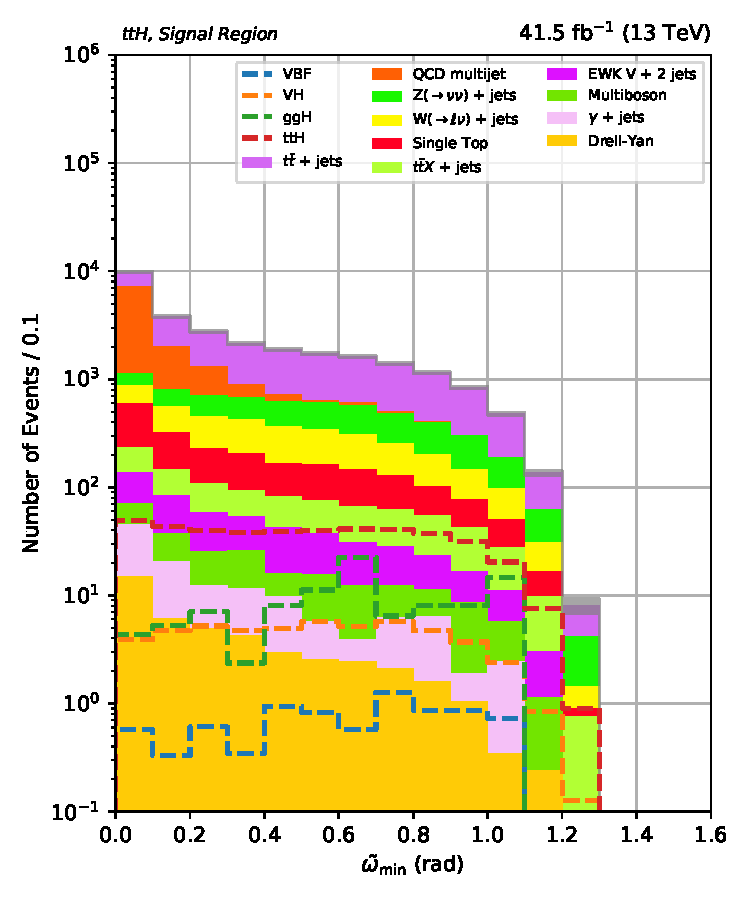
\includegraphics[width=\textwidth]{figures/category_optimisations/min_omega_tilde_ttH.pdf}
        \caption{\ttH category}
    \end{subfigure}
    \hfill
    \begin{subfigure}[b]{0.27\textwidth}
        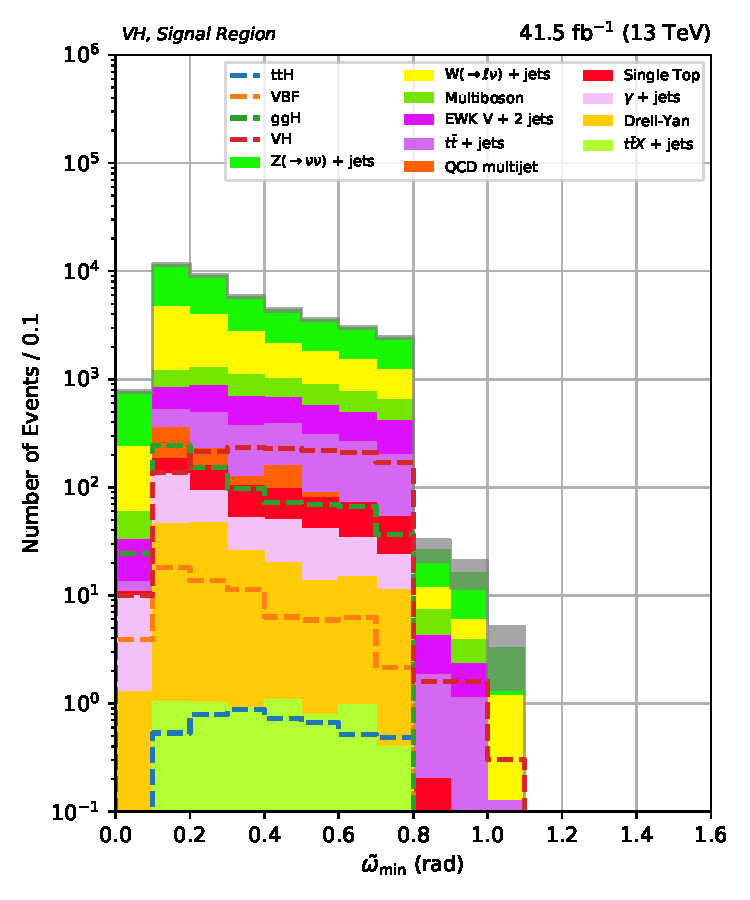
\includegraphics[width=\textwidth]{figures/category_optimisations/min_omega_tilde_VH.pdf}
        \caption{\VH category}
    \end{subfigure}
    \hfill
    \begin{subfigure}[b]{0.27\textwidth}
        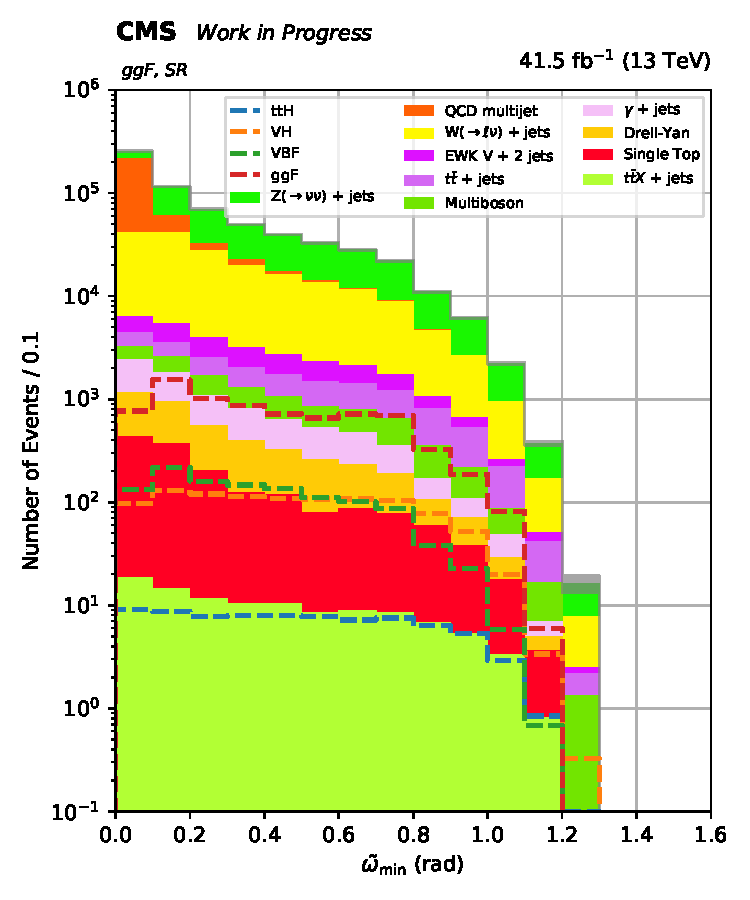
\includegraphics[width=\textwidth]{figures/category_optimisations/min_omega_tilde_ggH.pdf}
        \caption{\ggH category}
    \end{subfigure}

    \begin{subfigure}[b]{0.27\textwidth}
        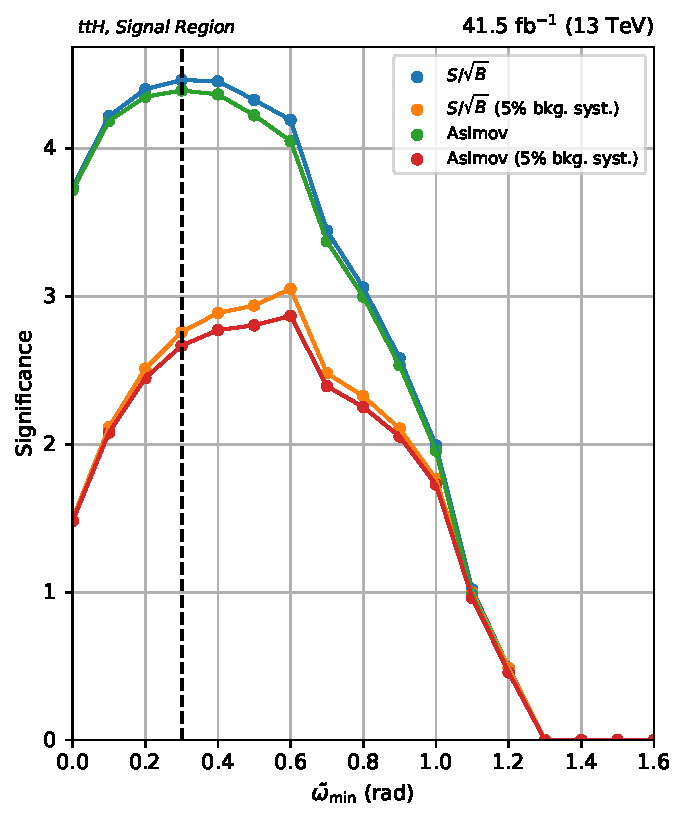
\includegraphics[width=\textwidth]{figures/category_optimisations/significance_ttH_min_omega_tilde_all.pdf}
        \caption{Significance of cut in \ttH category}
    \end{subfigure}
    \hfill
    \begin{subfigure}[b]{0.27\textwidth}
        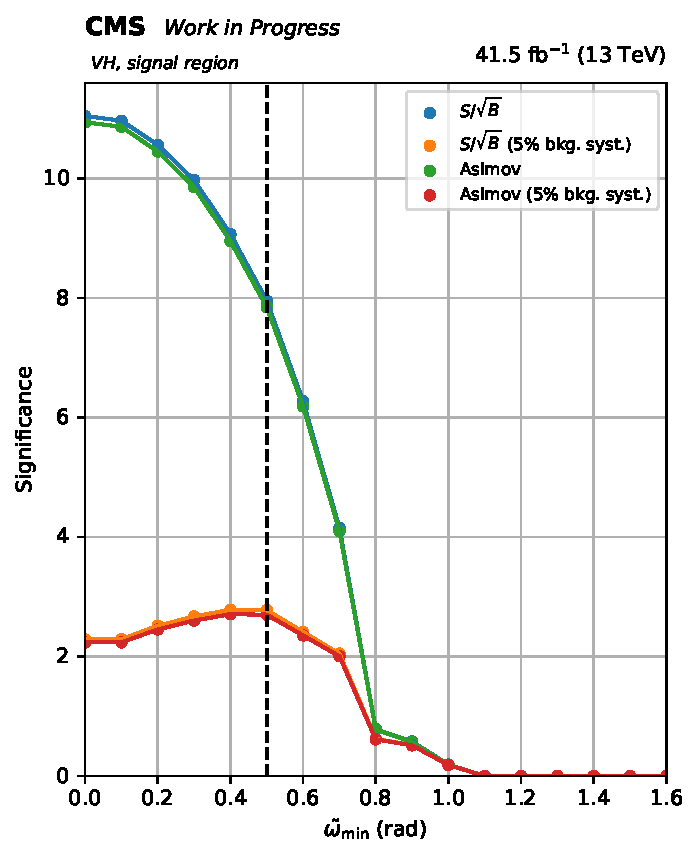
\includegraphics[width=\textwidth]{figures/category_optimisations/significance_VH_min_omega_tilde_all.pdf}
        \caption{Significance of cut in \VH category}
    \end{subfigure}
    \hfill
    \begin{subfigure}[b]{0.27\textwidth}
        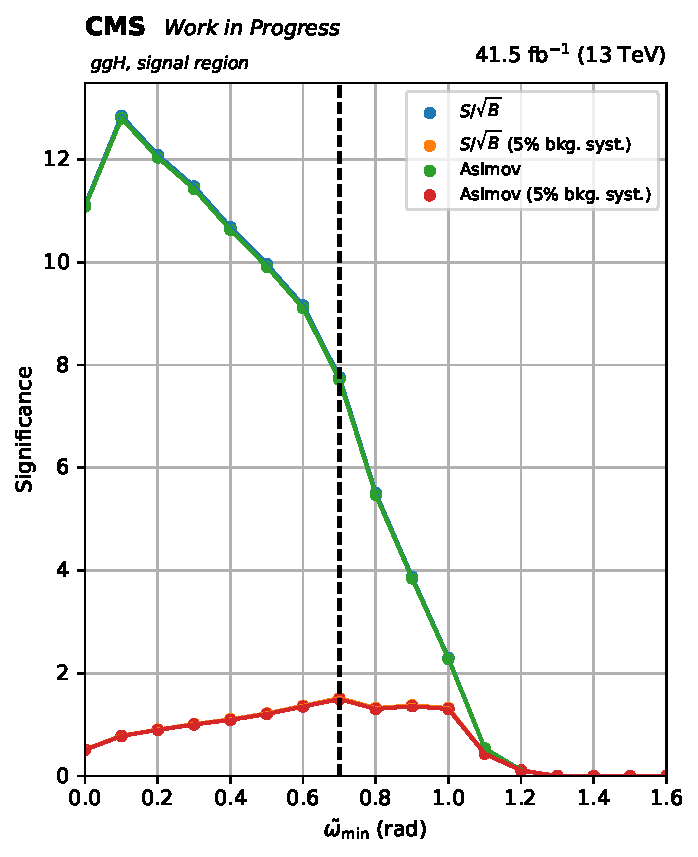
\includegraphics[width=\textwidth]{figures/category_optimisations/significance_ggH_min_omega_tilde_all.pdf}
        \caption{Significance of cut in \ggH category}
    \end{subfigure}
    \caption[Distributions of \omegaTilde in the signal region in the \ttH, \VH, and \ggH categories, along with the significance---using several figures of merit---if a cut is placed to the right of a given value]{Top row: distributions of \omegaTilde in the signal region in the \ttH, \VH, and \ggH categories. Bottom row: the significance---using several figures of merit---if a cut is placed to the right of a given value of \omegaTilde in each category. The black dotted line indicates the threshold used in the analysis. These are showcased after the analysis-level selection on signal and background simulation for the 2017 data-taking era.}
    \label{fig:htoinv_category_optimisations_significances}
\end{figure}

% Figures from 12th August 2020, scenario 5. When remaking, ensure the colours of the signal lines are consistent, and the legend doesn't overlap with the distribution

It is obvious that the shapes and magnitudes of the significance distributions are sensitive to the inclusion of an estimated systematic uncertainty. Increasing its size affects the shape little, though impacts the magnitude more significantly. In bins with high background occupancy, even a small systematic uncertainty can wash out traces of signal. The thresholds chosen for \omegaTilde do not necessarily maximise the significance---where the Asimov method with $\bkgsystuncert = \text{5\,\%}$ was the leading choice---but to sufficiently separate signal and background, while not removing too many events. The \glspl{CR} in the analysis perform better estimations of their responsible backgrounds when adequately populated. Reducing the background too greatly with the \omegaTilde cut can therefore cause problems in multiple aspects of the analysis.


%=========================================================


\subsection{Binning}
\label{subsec:htoinv_binning}

In addition to the categories above, events are placed in bins of \ptmiss as that distribution is expected to maximally differentiate signal and background in the final fit (see Chpt.~\ref{sec:htoinv_satistical_treatment}). Since the number of events can significantly differ between categories in the different regions of the analysis, a global binning configuration is inadequate. For each category, the number and widths of the bins are tuned to ensure sufficient statistical precision. These schemes are tied to the category, so are reflected in all regions such that transfer factors from the background estimation methods are calculated on a bin-by-bin basis.\footnote{Not sure if this subsection should instead go in the fit discussion. But as I haven't written any of that, I'll leave it here for now.}
